
\lhead[\chaptername~\thechapter]{\rightmark}

\rhead[\leftmark]{}

\lfoot[\thepage]{}

\cfoot{}

\rfoot[]{\thepage}

\chapter{Additional Results\label{Appen}}

The future work for our method on image classification task includes training on a bigger dataset. 
In figure \ref{fig:hier365}, an example hierarchy for classification task on Places365 dataset is obtained with artificially generated users.
We used 100 different user types, each with a random bias towards a subset of class labels. Number of biased labels for each user is randomly selected between 2 and 20. 
10 users are generated from each user types. This algorithm to generate users realistically is explained in section \ref{ssec:genusers}.

In section \ref{sec:FasterANN}, distribution of classification labels in 20 sub-spaces is shared. More detailed version with 100 sub-spaces can be examined in figure \ref{fig:100poslists}.

For our method in image retrieval task, parameters can be adjusted to have various results. 
One parameter controls the selection of sub-spaces to search in a way that a sub-space is chosen if it contains any of the user-required labels at least $k$ times. 
This parameter $k$ is called 'min-occur' in the figure \ref{fig:20randomcomb}. 
Although it is not practically possible to combine our method's best results, it is visualized in the figure.

Lastly, performance of our method on real-life data under different parameters can be seen in the figure \ref{fig:reallifeexp-all}. 
Because the number of user-required labels turned out to be quite large(73), some labels are discarded according to their classification probability or number of occurrences in the training images. 
However, the more the labels are discarded, the less the accuracy becomes.


\begin{figure}
    \centering
    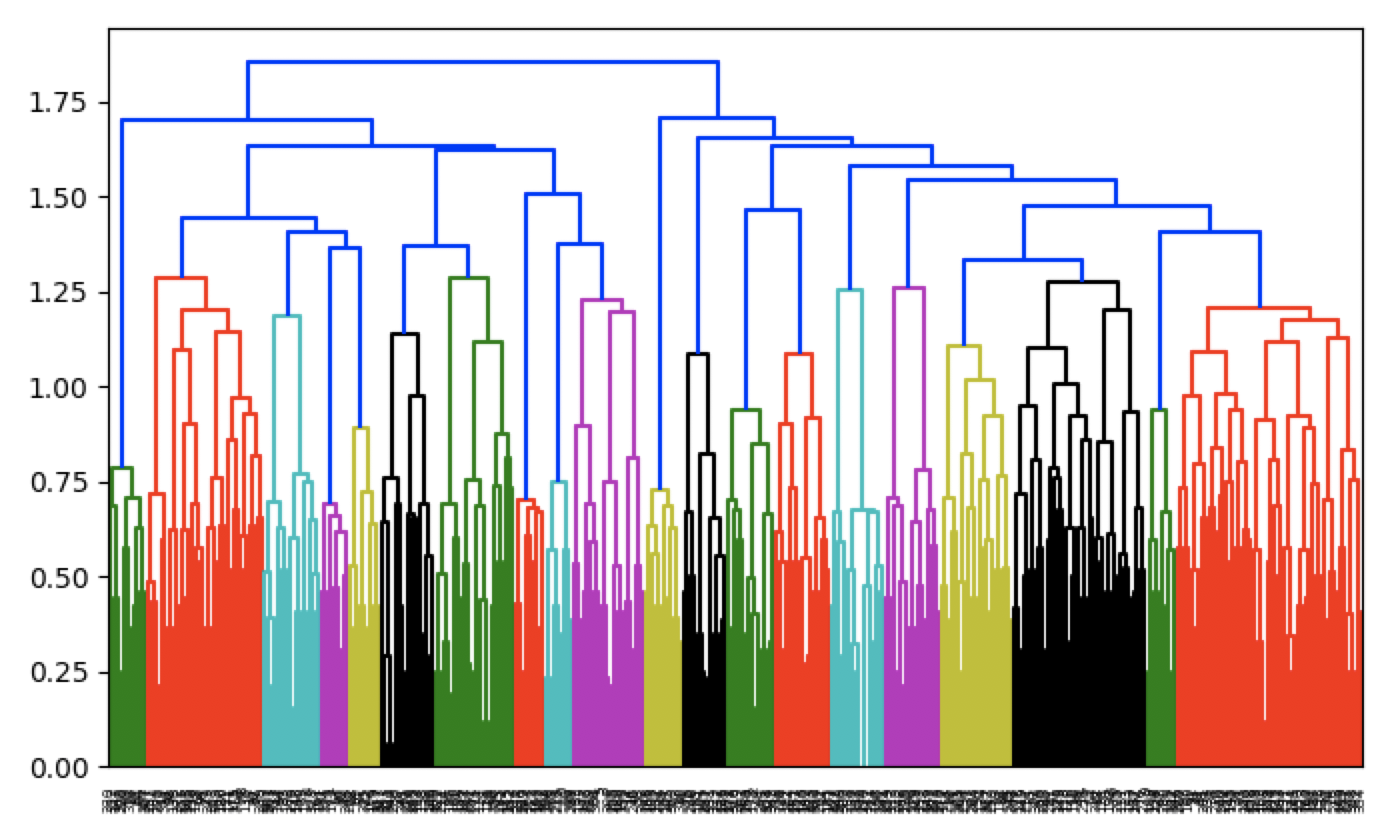
\includegraphics[width=\textwidth]{thesis/images/365class-hierarchy.png}
    \caption{Example hierarchy obtained for classification task on Places365 dataset}
    \label{fig:hier365}
\end{figure}

\begin{sidewaysfigure}[ht]
    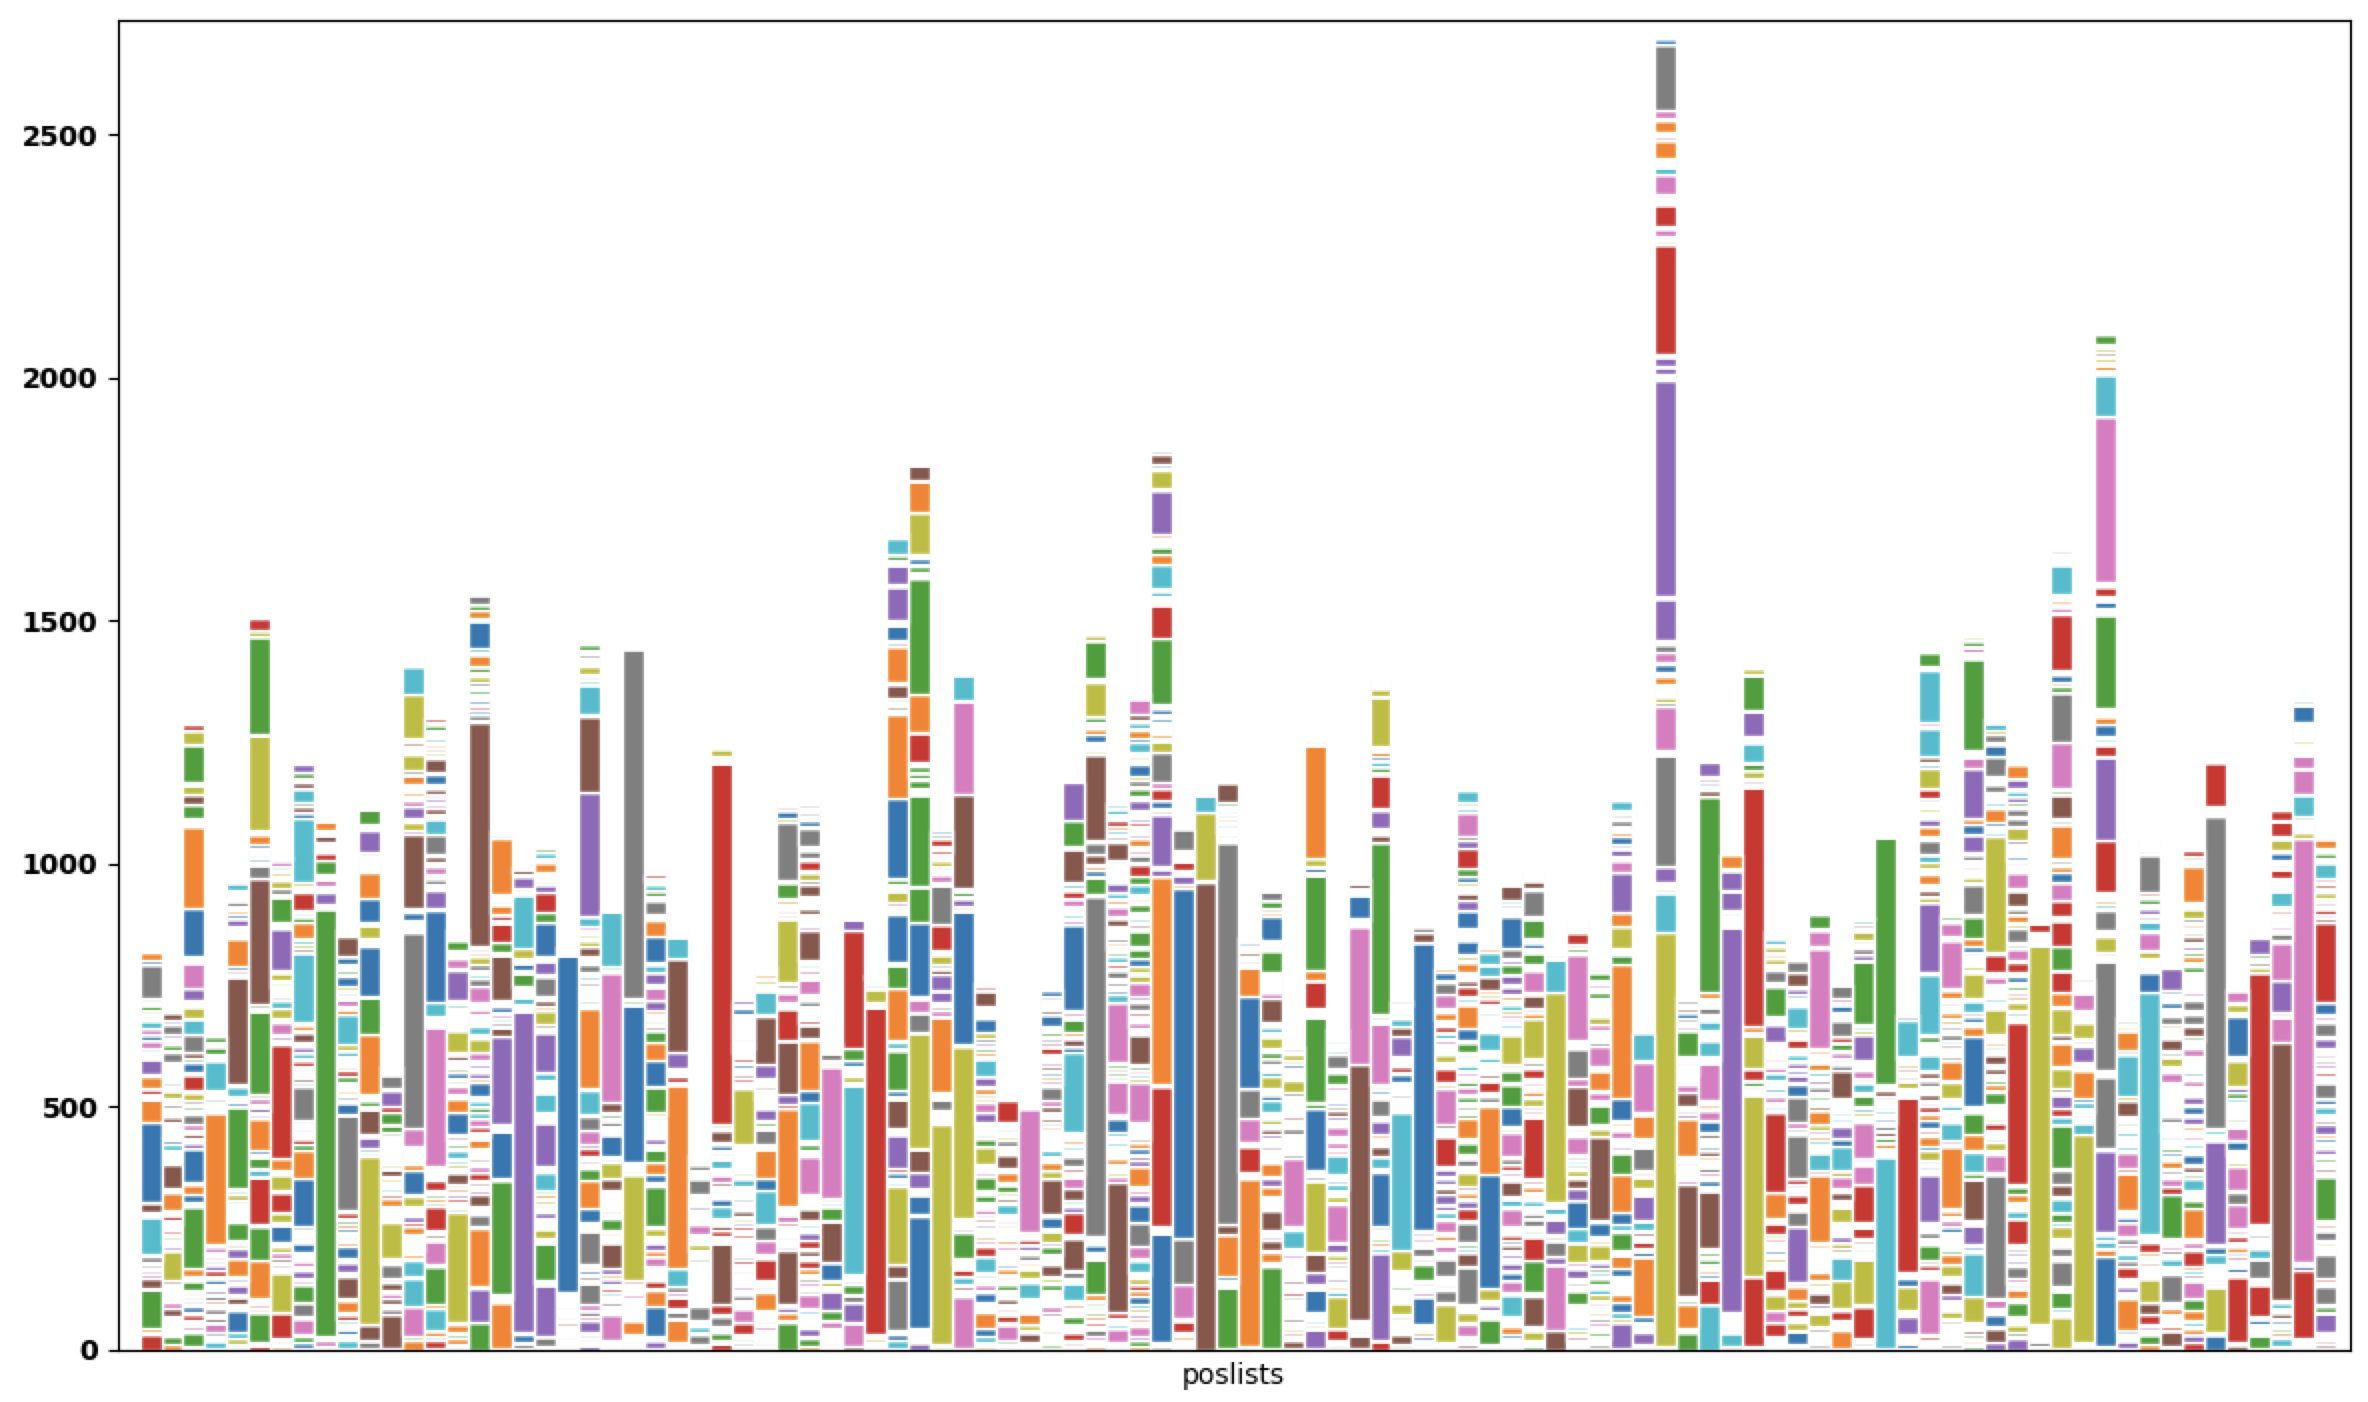
\includegraphics[width=\textwidth]{thesis/images/100poslists.png}
    \caption{More detailed classification label distribution to sub-spaces with 100 sub-spaces}
    \label{fig:100poslists}
\end{sidewaysfigure}

\begin{figure}
    \centering
    \begin{minipage}[b]{.5\textwidth}
        \centering
        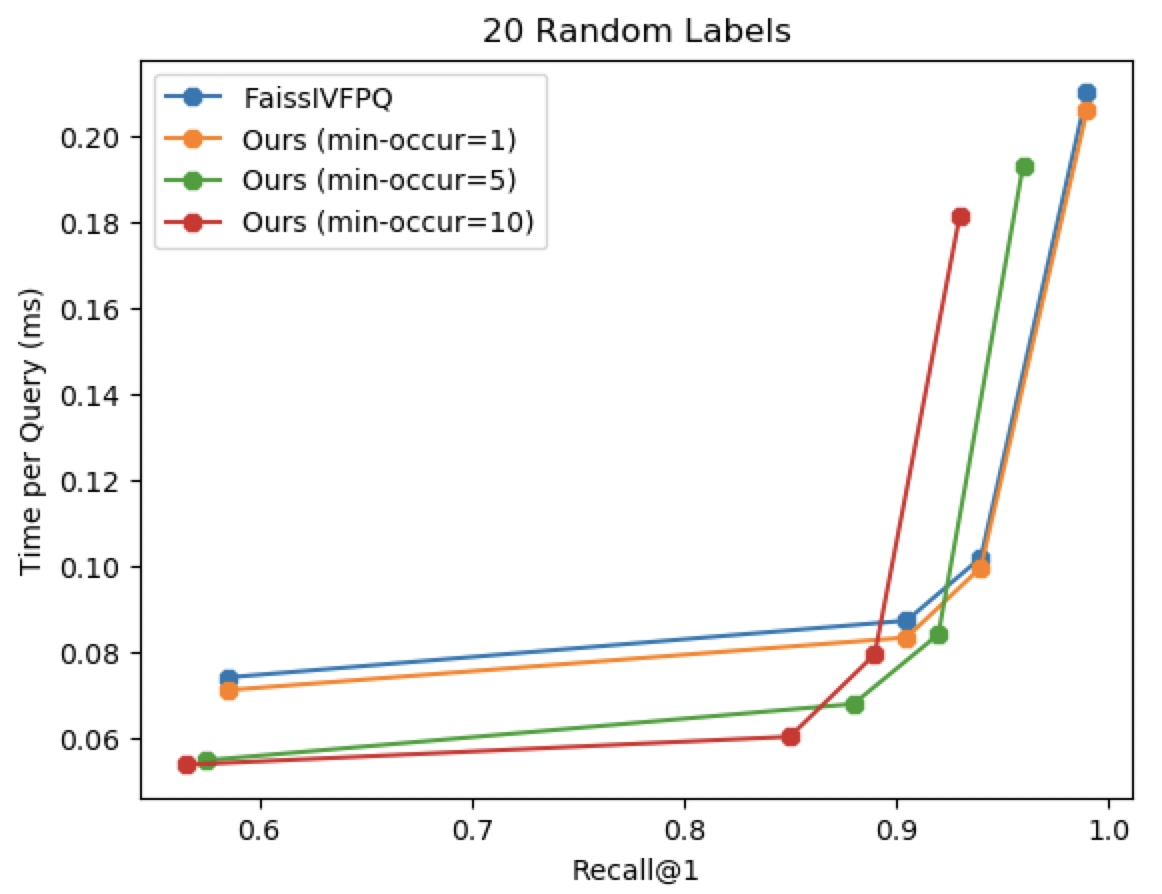
\includegraphics[width=.9\linewidth]{thesis/images/20random-all.png}
        % \caption{Results for 3 random label}
        % \label{fig:randomexpsub1}
    \end{minipage}%
    \begin{minipage}[b]{.5\textwidth}
        \centering
        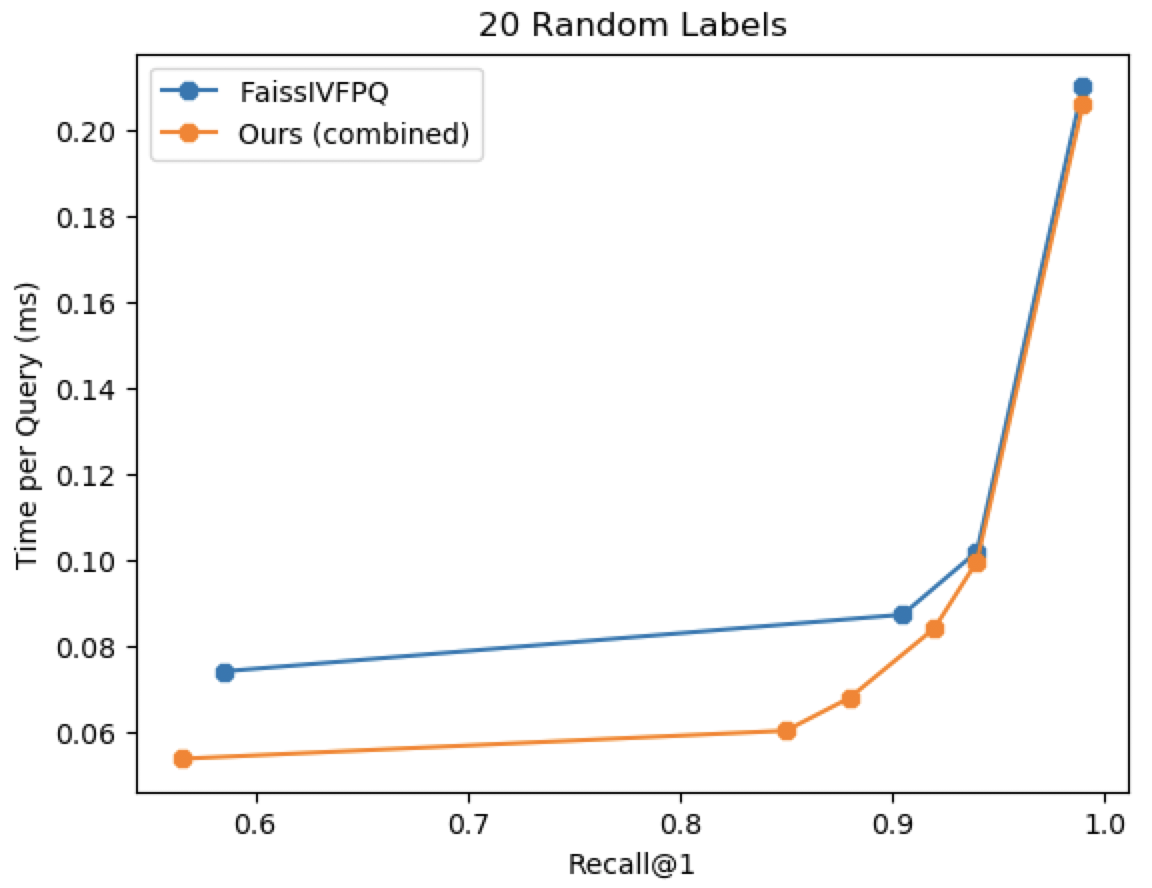
\includegraphics[width=.9\linewidth]{thesis/images/20random-combined.png}
        % \caption{Results for 10 random label}
        % \label{fig:randomexpsub2}
    \end{minipage}
    %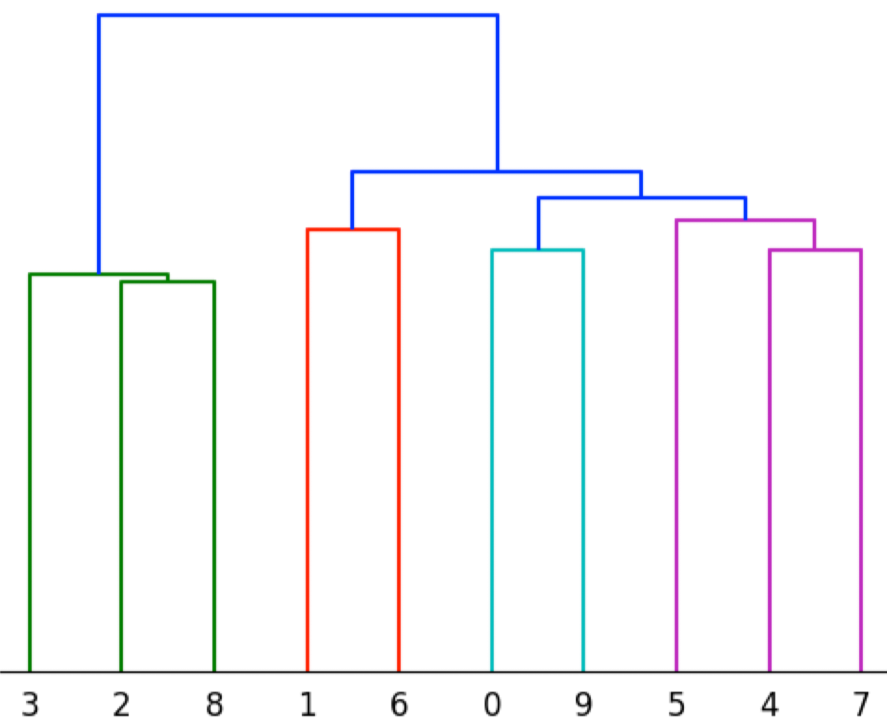
\includegraphics[width=0.40\textwidth]{images/hierfig.png}
    \caption{Combining our method's best results with different parameters}
    \label{fig:20randomcomb}
\end{figure}



\begin{figure}
    \centering
    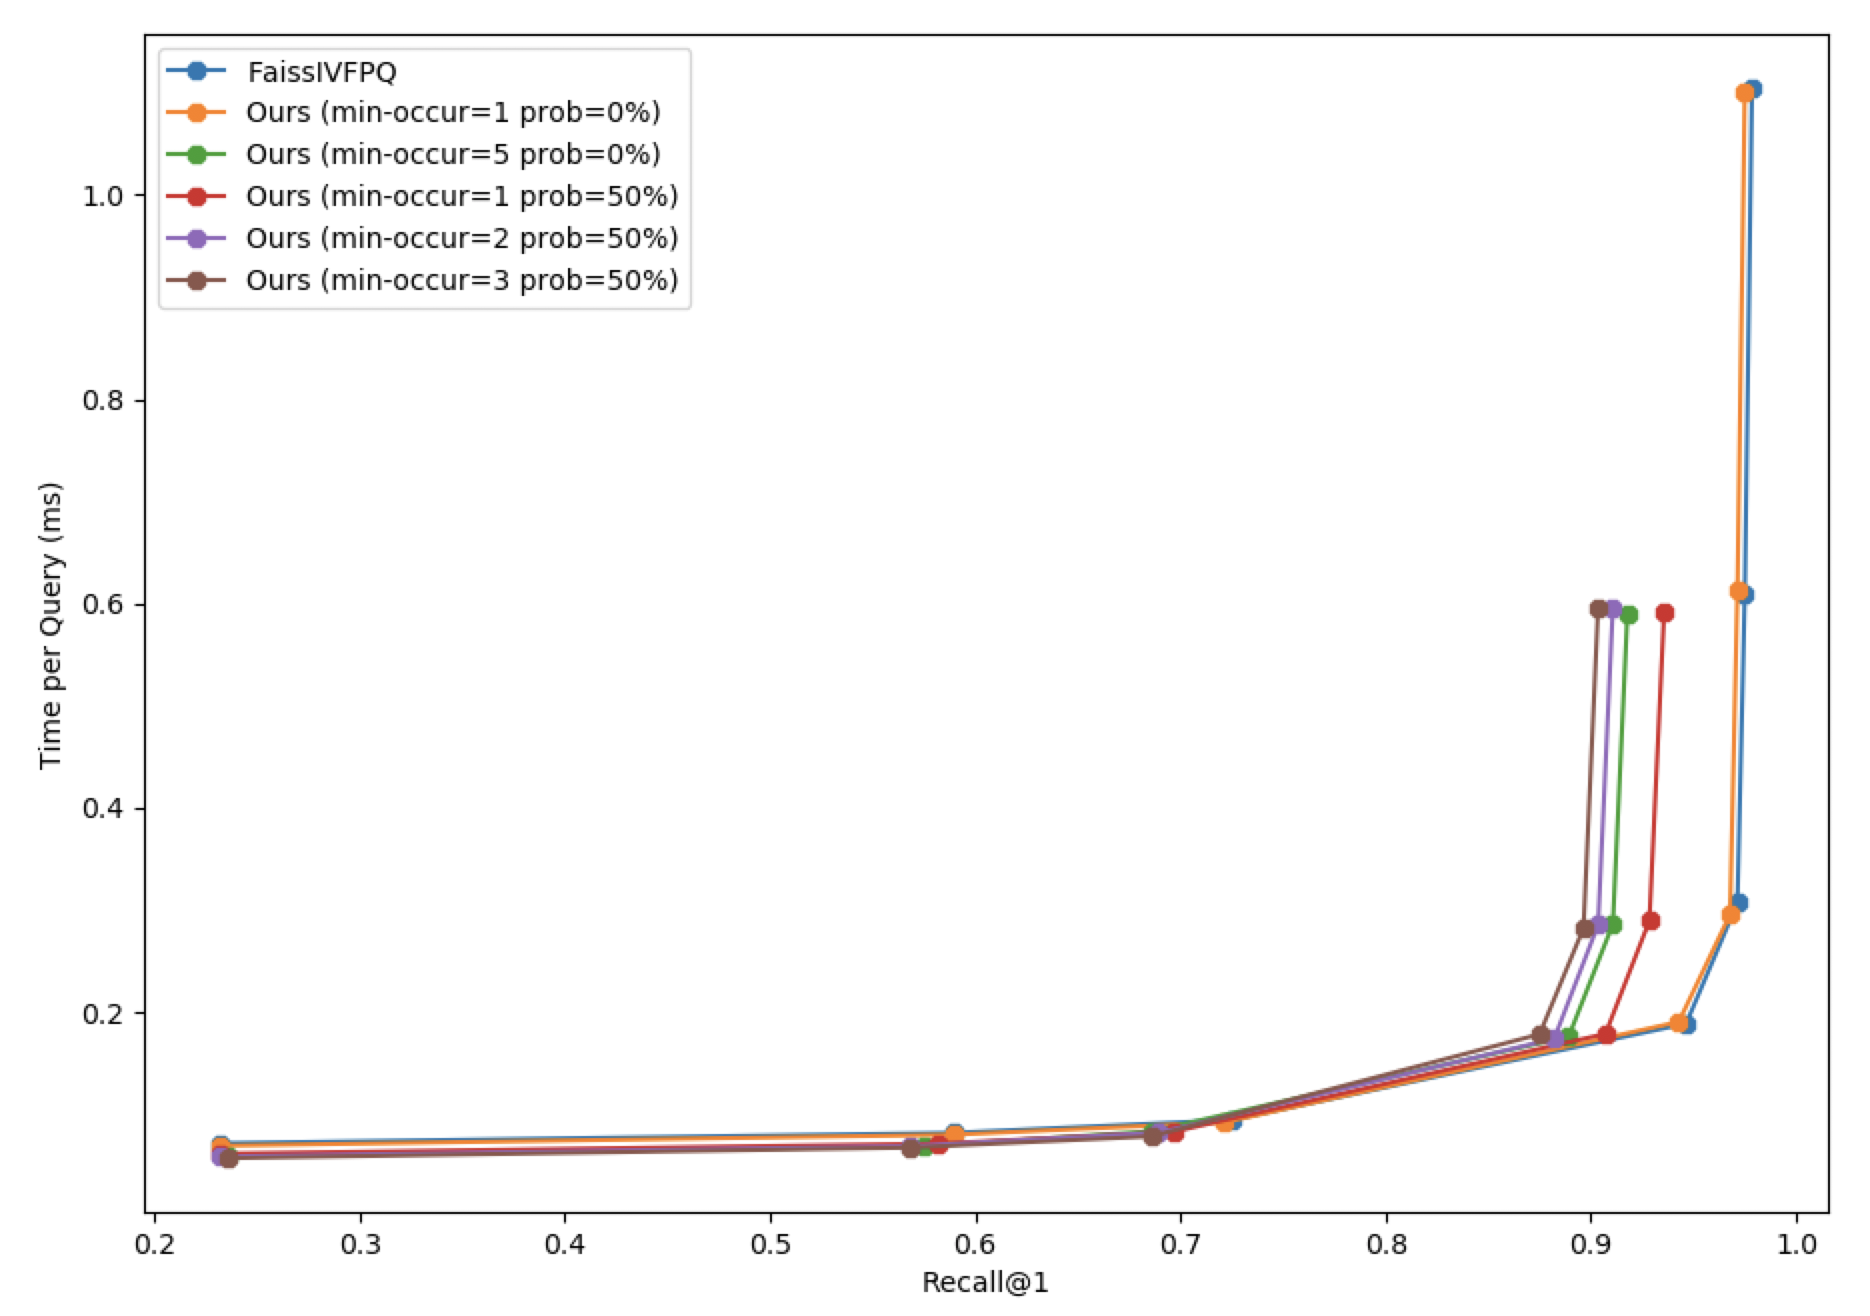
\includegraphics[width=\textwidth]{thesis/images/real-life-exp-all-ours.png}
    \caption{Results of our method on real-life data with different parameters }
    \label{fig:reallifeexp-all}
\end{figure}
